We discuss the MHD solver performance. We begin with the strong-scaling comparison:
\begin{enumerate}
\item For pure hydro results, Aurora and Frontier achieve about 80\% efficiency at $n/P \approx 4$M, consistent with earlier studies \cite{min23a}. 
\item For MHD, Aurorar leads Frontier, though MHD scaling is weaker despite using many of the same solvers. Considering a arge Frontier MHD run with $P = 72,000$ GCDs and $n \approx 662$B grid points, sustaining 0.114 TFLOPS per rank. The 3.3 s/step time—higher than the expected 1 s/step for hydro—is due to increased workload (two vector fields) and the need for stronger solvers for the magnetic field, with 37\% of time spent on coarse solves (10\% for velocity, 27\% for magnetic pressure).
\end{enumerate}

We were unable to scale the new MHD code on Aurora to the full machine due to some machine reliability issues, so Fig.~\ref{fig:pbli_1}(a) shows only hydro comparisons. Aurora is nearly 2$\times$ faster than Frontier at 72k accelerators but was unstable beyond 500 steps due to machine reliability issues. Nevertheless, it scales reasonably, with runtime decreasing by a factor of \~1.3 from 72k to 96k tiles, consistent with 80\% efficiency expected around $n/P \approx 3$–4M.

\begin{figure}
\centering
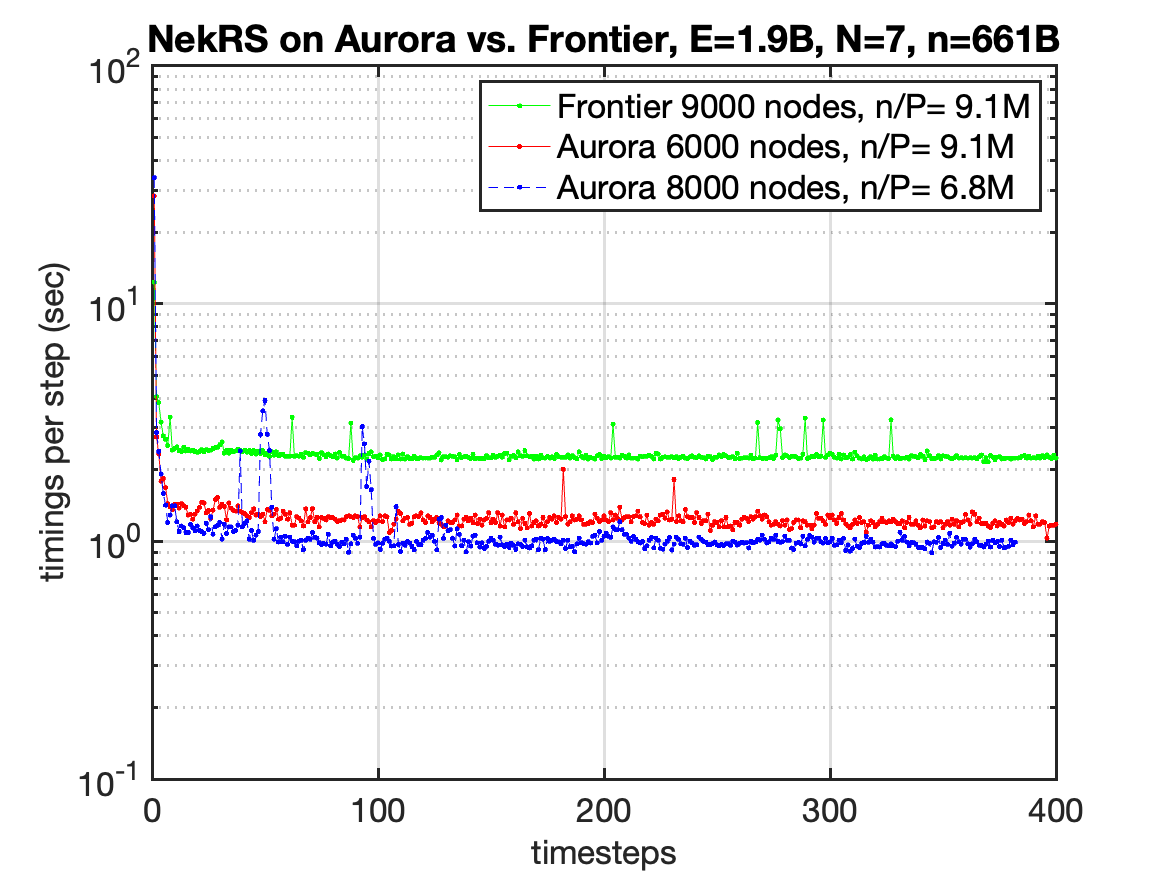
\includegraphics[width=3.in]{figs/time_tri_2_frontier_aurora.png}
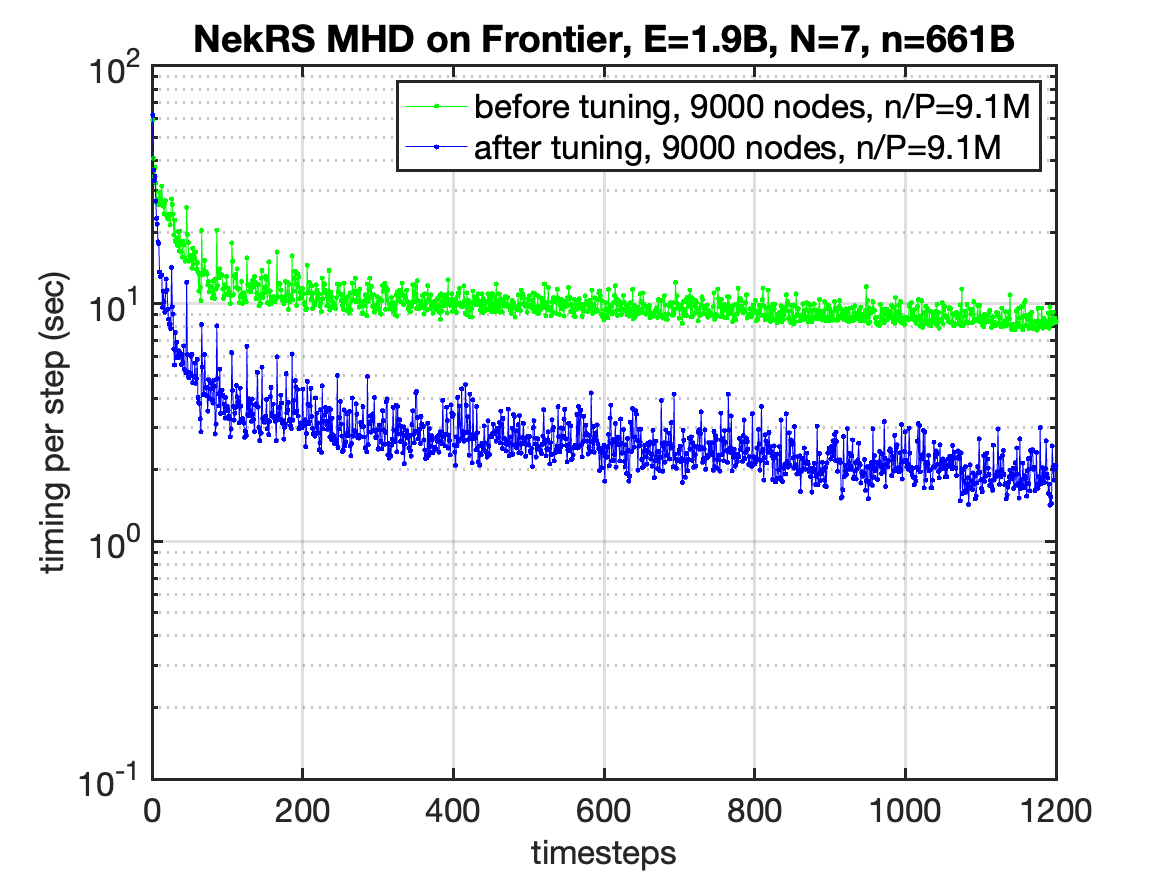
\includegraphics[width=3.in]{figs/mhd_time_lan_1.png}
\\
\hspace{0.3em} (a) \hspace{22.5em} (b)
\caption{\label{fig:pbli_1} NekRS runs on Aurora and Frontier: (a) Hydro-only at $P = 72{,}000$–$96{,}000$; (b) Frontier MHD performance before and after tuning.}
\end{figure}

Table~\ref{tab:simulation_metrics} compares throughput across cases. CHIMERA's complex geometry caused degraded performance in 2024 \cite{sc24}, but here we see significant recovery. Aurora achieves strong hydro throughput, while MHD on Frontier exceeds 2.5T DOFs/s—an order-of-magnitude gain over last year.

\begin{table}
\footnotesize
\setlength{\tabcolsep}{4pt}
\renewcommand{\arraystretch}{1.1}
\centering
\begin{tabular}{|l|c|c|c|c|c|c|}
\hline
& \textbf{SC23}~~\cite{sc23} & \textbf{CHIMERA}~~\cite{sc24} & \textbf{Aurora} & \textbf{Frontier} & \textbf{Frontier + MHD} & \textbf{Frontier + MHD + tuning} \\
\hline
Solid elements    & 937M  & 0     & 1.52B & 1.52B & 1.52B & 1.52B \\
Fluid elements    & 820M  & 1.69B & 405M  & 405M  & 405M  & 405M \\
Grid points       & 603B  & 1.23T & 662B  & 662B  & 662B  & 662B \\
DOFs              & 1.73T & 6.16T & 1.22T & 1.22T & 3.87T & 3.87T \\
Grid points/s     & 1.40T & 50.9B & 676B  & 300B  & 78.9B & 433B \\
DOFs/s            & 4.02T & 254B  & 1.24T & 552B  & 461B  & 2.53T \\
\hline
\end{tabular}
\caption{Simulation throughput across platforms and configurations.}
\label{tab:simulation_metrics}
\end{table}


